\newpage

\section{Bluetooth on the CircuitPlayground Bluefruit (CPB Only)}
\label{s:Bluetooth}

\subsection{Parts List}

\begin{enumerate}[itemsep=-5pt]
\item Smart Phone
\item Adafruit BLE Connect App (\href{https://play.google.com/store/apps/details?id=com.adafruit.bluefruit.le.connect}{Play Store}/\href{https://apps.apple.com/us/app/bluefruit-connect/id830125974}{App Store})
\item CircuitPlayground Bluefruit
\item USB Cable
\item Laptop
\end{enumerate}

\subsection{Learning Objectives}
\begin{enumerate}[itemsep=-5pt]
\item Understand the bluetooth module on the CircuitPlayground Bluefruit
\item Learn how to send data via the Bluefruit to your smart phone
\item Understand how to plot data sent via UART
\end{enumerate}

\subsection{Extra Help}

You might find plotting data via bluetooth to be rather difficult and it was pretty difficult for me until I learned that you can export data as a txt file rather than a csv file. Before I learned how to do that I put together a \href{https://www.youtube.com/playlist?list=PL_D7_GvGz-v0-U3JACRMgldvqQqn2mje9}{4 part series} describing everything in this module. Worst case you can just watch the \href{https://www.youtube.com/watch?v=9EHNFdVX9O8&list=PL_D7_GvGz-v0-U3JACRMgldvqQqn2mje9&index=3}{third video in the series}. The video is 30 minutes but the first 8 minutes goes through setting up the bluetooth module and the rest of the video is just on plotting the exported csv data which took me some time. Note that exporting data as a txt file is the preferred method as parsing the file is way easier.

\subsection{Getting Started}

In this module we're going to go over how to get the bluetooth module on the Circuitplayground Bluefruit (CPB). There is a lot you can do with bluetooth but the bottom line is that you can send data from your phone to your CPB and you can also send data to your smart phone. All code required for this module is on my \href{https://github.com/cmontalvo251/Microcontrollers/tree/master/Circuit_Playground/CircuitPython/CPB_DataLogger}{Github}.

First we're going to run the \href{https://github.com/cmontalvo251/Microcontrollers/blob/master/Circuit_Playground/CircuitPython/CPB_DataLogger/bluefruit_uart_send.py}{bluetooth\_uart\_send.py} script which sends data to your smart phone via something called UART which is a type of serial communication. It's beyond the scope of this lesson but serial is digital as opposed to analog like we will do in future videos. 
\begin{figure}[H]
  \begin{center}
    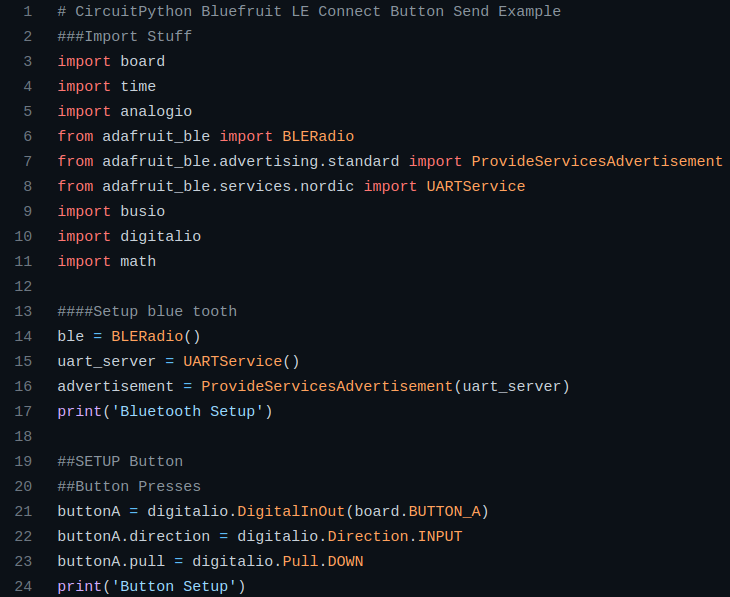
\includegraphics[width=\textwidth]{Figures/bluetooth_code.png}
  \end{center}
\end{figure}
Lines 4-14 import a ton of modules. You'll recognize many of them like analogio, thermistor, and lis3dh but the new ones are the ones that say ble. These are the bluetooth modules required for the CPB. Lines 22-24 setup the thermistor and lines 26-31 setup the accelerometer as we've done in another lesson. Lines 16-20 kick of the BLERadio object and the UARTService() to send data. That's the only required setup for this lesson. {\bf Note: The image below is from an old version o the code. On line 35 a new line of code has been added print('Look for',ble.name). ble.name is the name of your CPB which is unique to your device.}
\begin{figure}[H]
  \begin{center}
    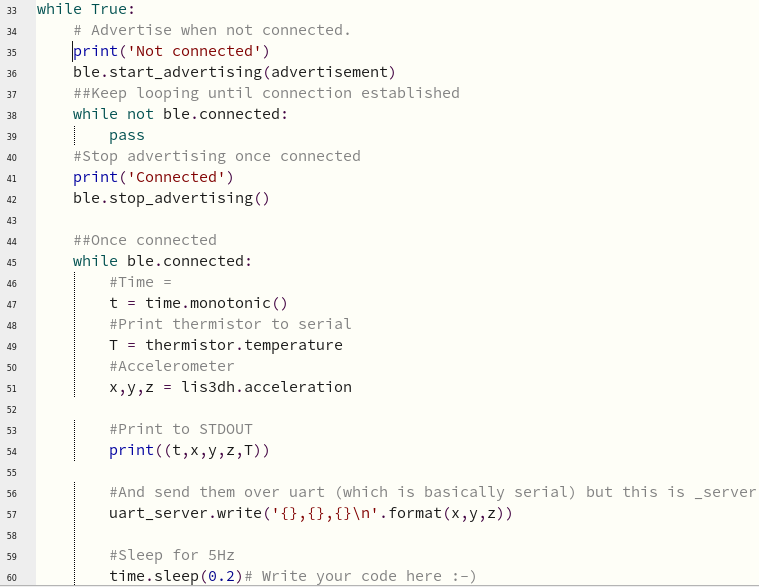
\includegraphics[width=\textwidth]{Figures/bluetooth_code1.png}
  \end{center}
\end{figure}
The code above is the infinite while loop which actually contains 2 while loops. Lines 33-42 check to see if bluetooth is connected. If bluetooth is not connected it will start advertising to any devices that are listening. It will then enter a while loop from 38-39 until bluetooth is connected. Once bluetooth is connected it will enter into the second while loop from line 45-60. In those lines 47-54 is responsible for taking all the necessary measurements and printing them to the serial monitor in Mu. Line 57 send the data over bluetooth using the UART server. You'll notice in this case I'm sending x,y,z by using the format variable an the 3 empty {} brackets. If you want to send more data you need to add more empty brackets and more variables to the format function. When you first save this script your CPB will not be connected and enter into an infinite while loop where it waits for your smart phone to connect. If you open your smart phone and open the Bluefruit Connect App the following screen will pop up.
\begin{figure}[H]
  \begin{center}
    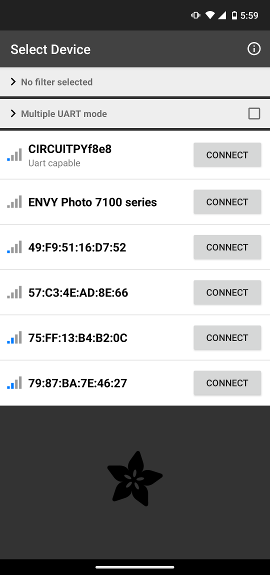
\includegraphics[width=0.3\textwidth]{Figures/phoneapp1.png}
  \end{center}
\end{figure}
In this case there are numerous different bluetooth modules can be seen but the one you need to click is the one that says CIRCUITPYf8e8. You will have a different code after CIRCUITPY and you can figure out what your 4 digit code is by making sure you have the {\it print('Look for',ble.name)} in your code. Once you do that the CPB will begin sending x,y,z accelerometer data to the smart phone. 
\begin{figure}[H]
  \begin{center}
    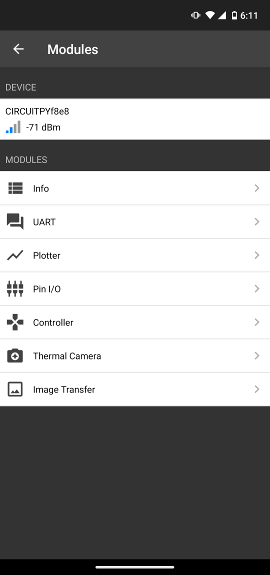
\includegraphics[width=0.3\textwidth]{Figures/phoneapp2.png}
  \end{center}
\end{figure}
There are numerous items you can click. The Controller is very fun for creating a remote control robot but we're only going to go over the UART and Plotter tabs. If you click the plotter tab you will be greeted with a live screen of the data being sent.
\begin{figure}[H]
  \begin{center}
    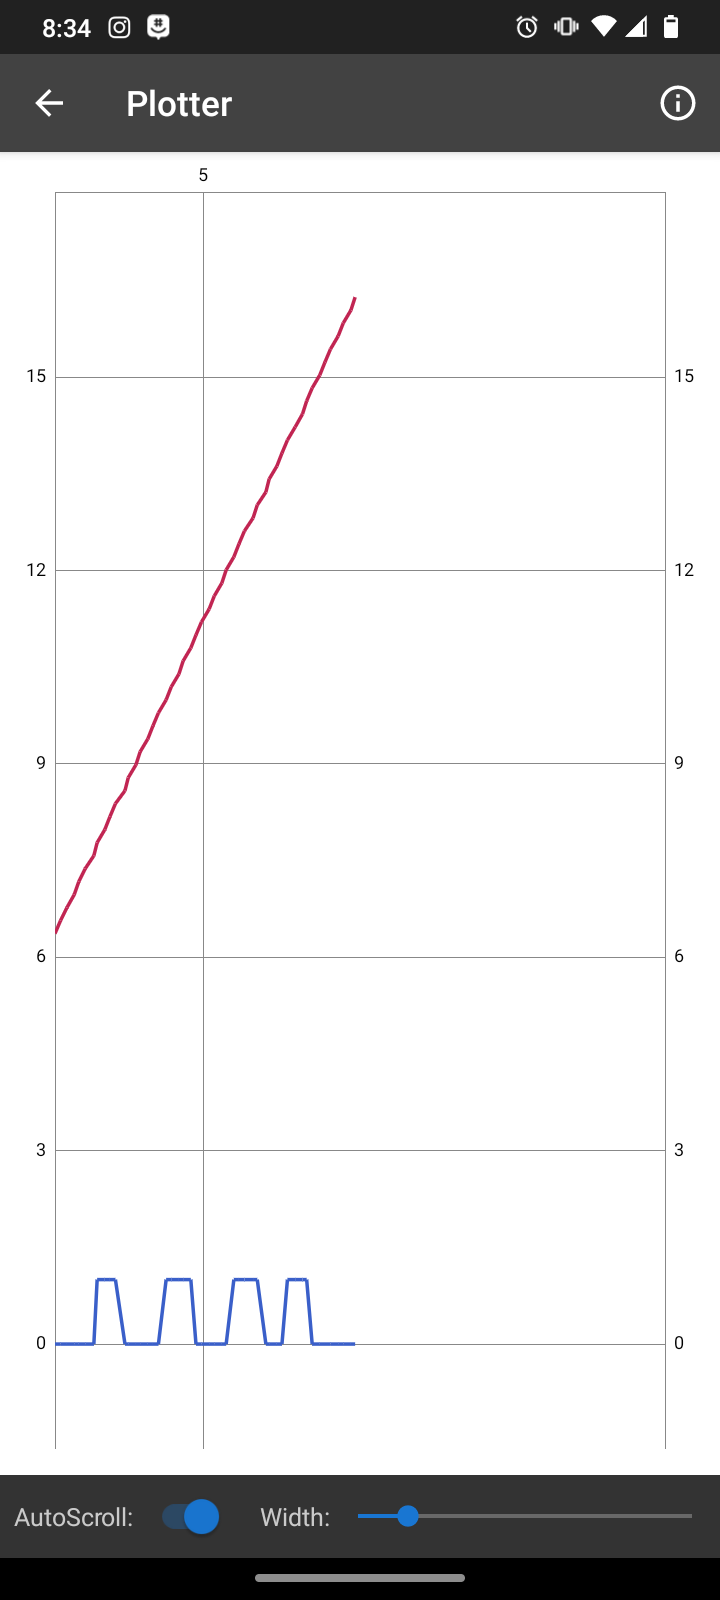
\includegraphics[width=0.3\textwidth]{Figures/phoneapp3.png}
  \end{center}
\end{figure}
In the photo above you can see three data streams that is coming directly from the CPB. This is great for live demonstrations and for debugging if you need to see data from an experiment and you don't have access to a laptop with Mu. If you hit the back arrow and then click UART you will see the raw data come in as text.
\begin{figure}[H]
  \begin{center}
    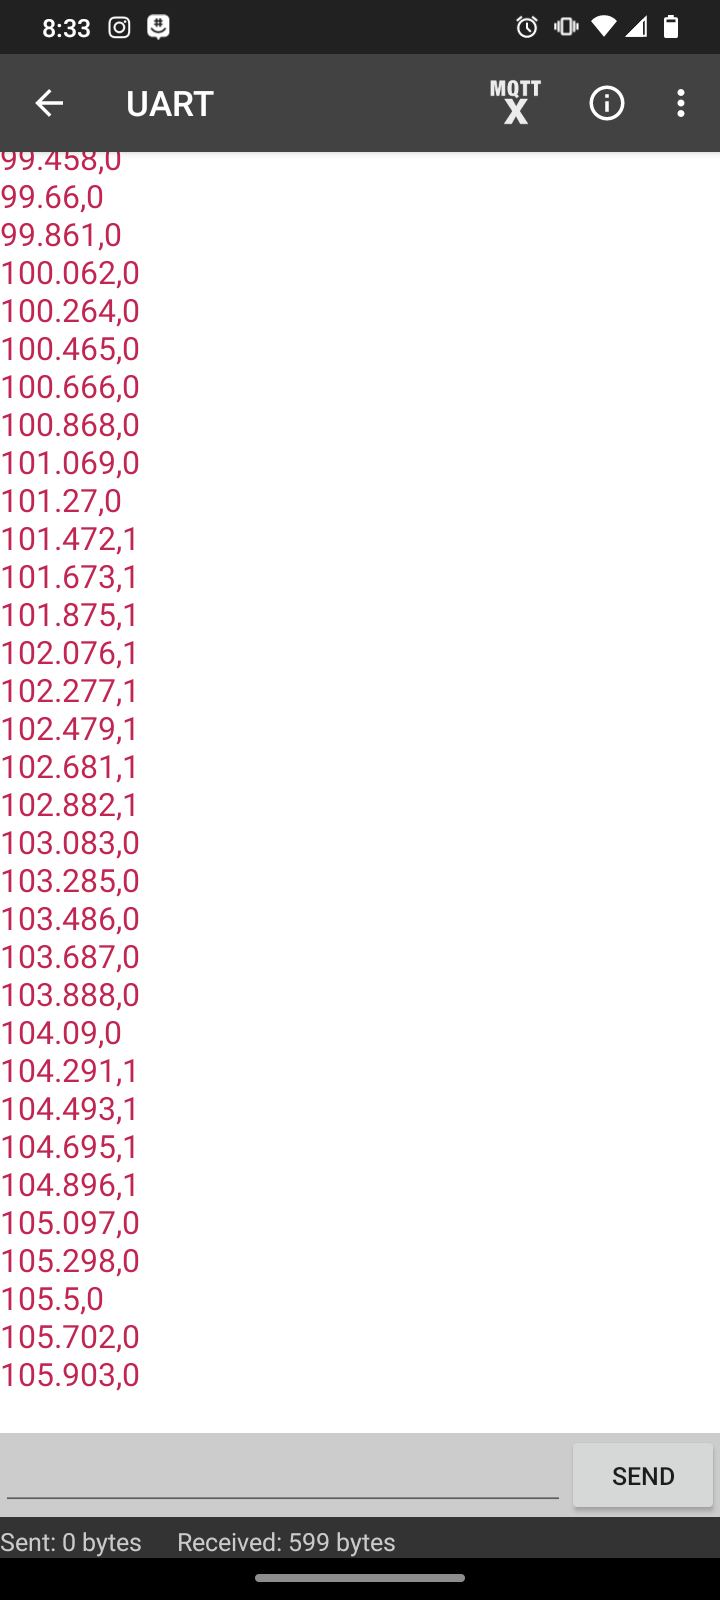
\includegraphics[width=0.3\textwidth]{Figures/phoneapp4.png}
  \end{center}
\end{figure}
Again here you can see the 3 data streams separated by commas. The very neat thing with the UART tab is that you can click the three vertical dots in the upper right hand corner and click export to TXT. The easiest thing for me was to export the data to google drive and then download the data to my computer. Before I downloaded the data though I went back and changed the following line of code
\begin{verbatim}
uart_server.write('{},{},{}\n'.format(x,y,z))
\end{verbatim}
to 
\begin{verbatim}
uart_server.write('{},{},{},{},{}\n'.format(t,x,y,z,T))
\end{verbatim}
In this case I added more empty brackets and also added the time and the temperature. When I opened the UART tab I was greeted with 6 data streams separated by commas. Once I downloaded the TXT file to my computer and opened it the data file looked like this.
\begin{figure}[H]
  \begin{center}
    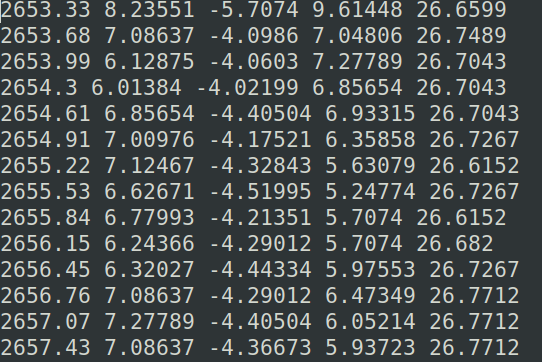
\includegraphics[width=0.8\textwidth]{Figures/csv_fileapp.png}
  \end{center}
\end{figure}
If you export the file as a CSV the data file will look completely different and it's much more complicated to plot. If you export the data as a TXT file you just need to use the np.loadtxt command to read in the data. Note you might have commas in your data file. If there are commas just use the CTRL+H command and replace all commas with spaces or use the np.loadtxt('file.txt',delimiter=',') command. Here's a simple piece of code to plot temperature and the accel data. I have not uploaded this code to Github simply because the code is very simple to create on your own.
\begin{figure}[H]
  \begin{center}
    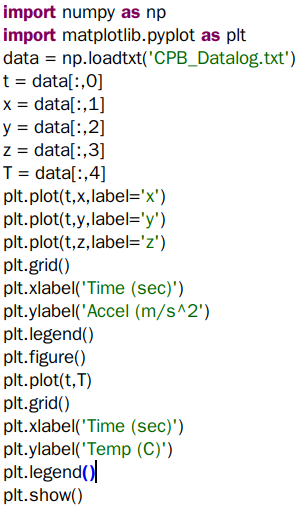
\includegraphics[width=0.5\textwidth]{Figures/phoneapp_plotcode.png}
  \end{center}
\end{figure}
The code reads in the data with the np.loadtxt command and then extracts each column. Once that's done the code plots all the data. In my case this was the result.
\begin{figure}[H]
  \begin{center}
    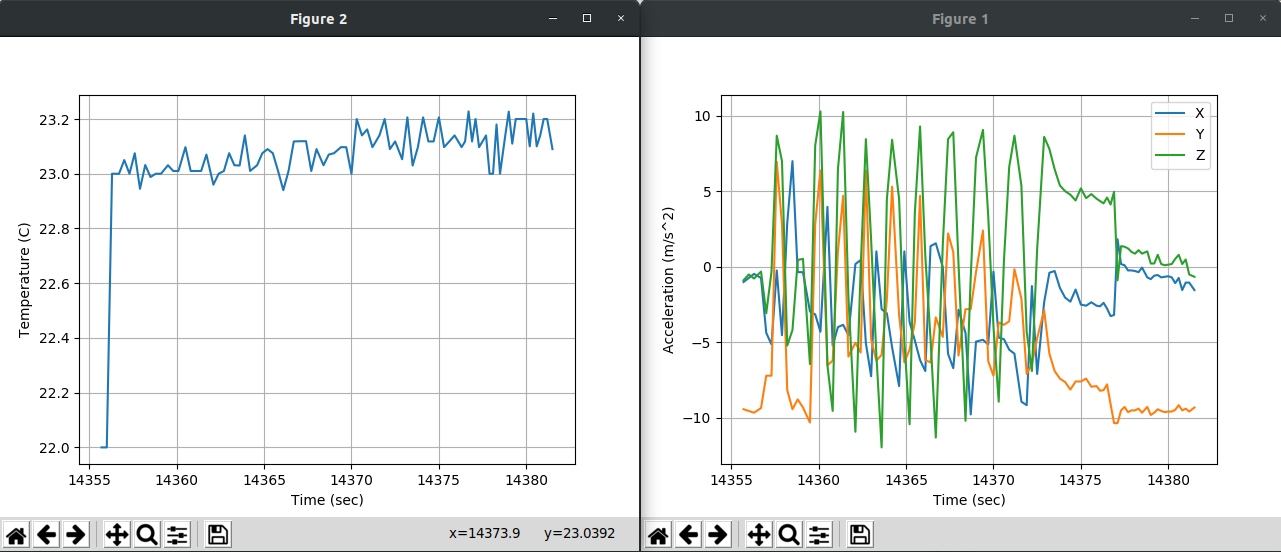
\includegraphics[width=\textwidth]{Figures/phoneapp_plots.png}
  \end{center}
\end{figure}

\subsection{Assignment}

Once you've done that upload a PDF with all of the photos and text below included. My recommendation is for you to create a Word document and insert all the photos and text into the document. Then export the Word document to a PDF. For videos I suggest uploading the videos to Google Drive, turn on link sharing and include a link in your PDF.
\begin{enumerate}[itemsep=-5pt]
\item First get the bluetooth code on your CPB and connect your smart phone to it and video tape yourself connecting the CPB to your smart phone (20\%)
\item Take a screenshot of the Plotter on your phone (15\%)
\item Take a screenshot of the UART raw data on your phone (15\%)
\item Export time, accelerometer and temperature data to a TXT file and plot it on your computer. Include your raw data in an appendix (20\%)
\item Include two plots: one of temperature and the other of acceleration like the lesson did above (30\%)
\end{enumerate}